\documentclass{sig-alternate}

% *** SPECIALIZED LIST PACKAGES ***
%
\usepackage{algorithmic}

\usepackage{array}

% *** PDF, URL AND HYPERLINK PACKAGES ***
%
\usepackage{url}

\begin{document}

% Copyright
\setcopyright{acmcopyright}
%\setcopyright{acmlicensed}
%\setcopyright{rightsretained}
%\setcopyright{usgov}
%\setcopyright{usgovmixed}
%\setcopyright{cagov}
%\setcopyright{cagovmixed}

%Conference
\conferenceinfo{GECCO '16}{Denver, CO, USA}
% --- End of Author Metadata ---

\title{Visualizing for success: making the user more efficient in
  interactive evolutionary algorithms}
%
% You need the command \numberofauthors to handle the 'placement
% and alignment' of the authors beneath the title.
%
% For aesthetic reasons, we recommend 'three authors at a time'
% i.e. three 'name/affiliation blocks' be placed beneath the title.
%
% NOTE: You are NOT restricted in how many 'rows' of
% "name/affiliations" may appear. We just ask that you restrict
% the number of 'columns' to three.
%
% Because of the available 'opening page real-estate'
% we ask you to refrain from putting more than six authors
% (two rows with three columns) beneath the article title.
% More than six makes the first-page appear very cluttered indeed.
%
% Use the \alignauthor commands to handle the names
% and affiliations for an 'aesthetic maximum' of six authors.
% Add names, affiliations, addresses for
% the seventh etc. author(s) as the argument for the
% \additionalauthors command.
% These 'additional authors' will be output/set for you
% without further effort on your part as the last section in
% the body of your article BEFORE References or any Appendices.

\numberofauthors{2} 
\author{
\alignauthor
Juan-J.~Merelo, \titlenote{Corresponding author}\\
\affaddr{Dept. of Computer Architecture and Technology and CITIC}\\
\affaddr{University of Granada, Granada, Spain} \\
\email{jmerelo@ugr.es}
\alignauthor
Mario Garc\'ia-Valdez, 
\affaddr{Dept. of Graduate Studies}\\
\affaddr{ Instituto Tecnol�gico de Tijuana, Tijuana, M\'exico}\\
}

\maketitle

\begin{abstract}

Using volunteer's browsers as a computing resource presents several
advantages, including cost, but it remains a challenge to fully harness the browser's
capabilities and to model the user's behavior so that those
capabilities can be leveraged optimally. One of the main challenges,
and heretofore not addressed, is how to first keep the user engaged in
the experiment so that his computation time is maximized, and second
how to present the information in such a way that it can be a call to
action that can, actually, help the evolutionary algorithm itself by
doing any number of operations on it. This paper is not a presentation
of results, but rather a call for comments to find out how to address
these problems in the most systematic way. 

\end{abstract}

\keywords{Volunteer computing, distributed computing, cloud computing,
visualization}


%---------------------------------------------------------------
\section{Introduction}

In volunteer computing systems, one of the objectives is to get the
user give as much time as possible to the experiment. Most of the
efforts nowadays include gamification, but these have the problem that
a competition has an implicit incentive to cheat to get ahead of your
competitors. 

In the case of systems such a NodIO \cite{2016arXiv160101607M}, which
is a minimal infrastructure to support pool-based distributed
evolutionary computing experiments, there is another issue with the
user. NodIO has been used for volunteer computing experiments by
embedding an island-based evolutionary algorithm inside a web page and
making them interchange information via the NodIO server, in a
spontaneous and eventually panmictic distributed evolutionary
algorithm. In the experiments we have carried out so far we have
realized that the way the user perceives the state of the algorithm
can make him or her act in several ways. For instance, reloading the
page, in which case a new population will be generated, with the best
individuals being sent to the pool adding to the diversity of that
pool. The user can also load the webpage in several browsers or
browser tabs so that it is adding more power and seeing how the
solution spreads from one to the other. In any case, we have noticed
that the user spontaneously is making it an {\em interactive}
algorithm, by applying {\em hypermutation} operators or even {\em
  distributing} themselves the population if their machine performance
allows them to do so. 

However, it will be impossible for the user to perceive what is
happening if the visualization does not convey that information in a
way that can be first understood by anyone without using any technical
term and second does not add too much overhead to the algorithm
itself. 

As far as we know, the problem of visualizing an evolutionary
algorithm so that the non-technical and spontaneous user can help it
find the solution faster has not been solved. We have made several
attempts that we will present in this paper, but this paper is
basically a request for comments during the workshop and later on so
that the scientific community understands the basis of this problem
and can also design their own solutions for it.  

That is why the rest of the paper will be devoted to a short state of
the art, an exposition of our efforts so far and finally instead of
conclusions several research questions that we hope are the bases for
a discussion of this issue.



%---------------------------------------------------------------
\section{State of the art}
\label{sec:soa}

As far as we have been able to find, there is no research devoted
exclusively to visualization to maximize involvement and interactivity
in volunteer computing experiments. From the very beginning,
BOINC@home included visualization of the results of the computation
\cite{anderson2006designing}, but it was only for informative
purposes, not a part of the system itself. 

There has been, however, a certain amount of research in interactive
evolutionary algorithms, where users perform all or some evolutionary
operations; in our case, since the
user has control of the browser, there is a limited amount of
interaction with it, namely, the fact that by reloading the webpage they
can apply a kind of hypermutation, killing the current population and
generating new individuals some of which will make their way to the
common pool via migration. In that sense, volunteer computing is also
a way of {\em human computation} \cite{quinn2011human}, a concept that
has also been applied to evolutionary algorithms \cite{972056, Nickerson2013}, in
this case extensively and with all operators. In general, these type
of human based evolutionary algorithms must be constrained to those in
which the problem representation can be understand by us;
\cite{cheng2004interactive} mentions evolution of text messages and
applies it to evolution of colors, where users have to pick up two
colored blocks to perform crossover; this is later on extended to the
OneMax problem, comparing the performance of a human operator who does
not know the shape of the fitness function with that of an interactive
evolutionary algorithm where the user himself is the one that acts as
fitness evaluator.

However, the visualization performance or the evolutionary algorithm itself is
eschewed in all the problems presented above, so that the only hint
that the user has of how the algorithm is doing is the fitness itself
or, even, just a hint of how close the user is to his desired
value. This is the problem we have been trying to solve and we will
show our solutions below, before calling for others in the last part
of the paper. 

\section{Description of the system and some results}
\label{sec:res}

NodIO \cite{2016arXiv160101607M,DBLP:conf/gecco/GuervosG15} is a
web-services based system that allows to run distributed evolutionary
computing experiments, including volunteer computing systems, with a
low overhead. 

The common part of all algorithms is the server, that has been
published with a free license in GitHub, which includes several REST
(Representational state transfer)
routes, which are remote procedure calls using the HTTP (Hypertext
Transfer Protocol). In practice, that means that clients use a
standard and well known interface, HTTP, to communicate with it and
clients can be written in many different languages, including
JavaScript on the client  or Perl. 

The server receives individuals from the client using the {\tt PUT}
HTTP command. The individual received is stored in a cache that is
refreshed in sub-second intervals, currently set at 0.2 seconds, and
has a finite size equal to 32, although it can have a few elements
more before the refreshing period. The cache is renovated in a First
In, First Out fashion, which, from the point of view of the
evolutionary algorithm, contributes to the diversity of the stored
population. In general, this way of using a stored population from
which some individuals are drawn is called a pool-based evolutionary
algorithm
\cite{pool:ga,bollini1999distributed,gong2015distributed, sofea:evopar2012,DBLP:journals/grid/ValdezTGVO15,garcia2014unreliable,LNCS86720702, DBLP:conf/3pgcic/GuervosMFEL12,sofea:naco}
 stores them and returns a random individual from the
store and some more information. 

\begin{figure*}[!htb]
\centering
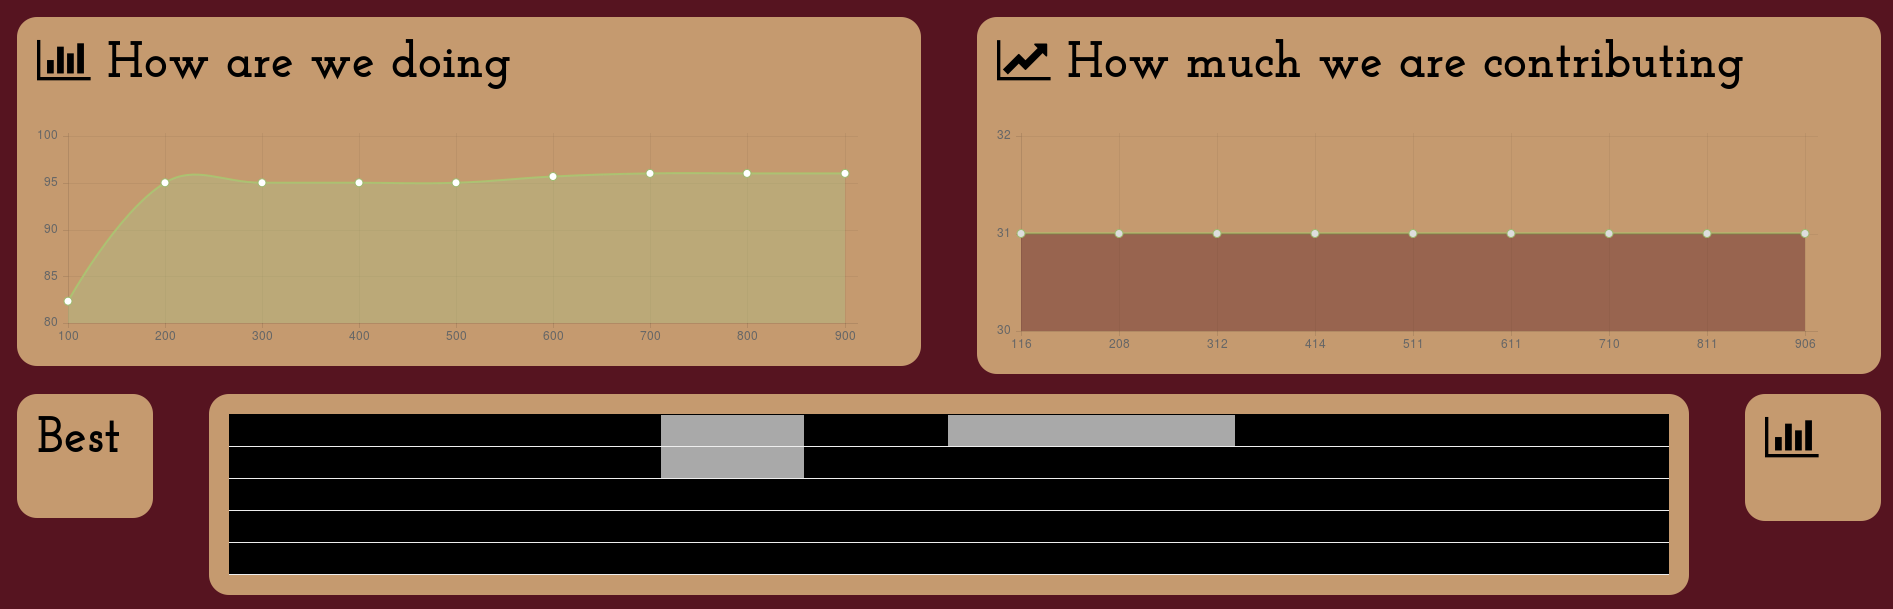
\includegraphics[width=0.95\linewidth]{all.png}
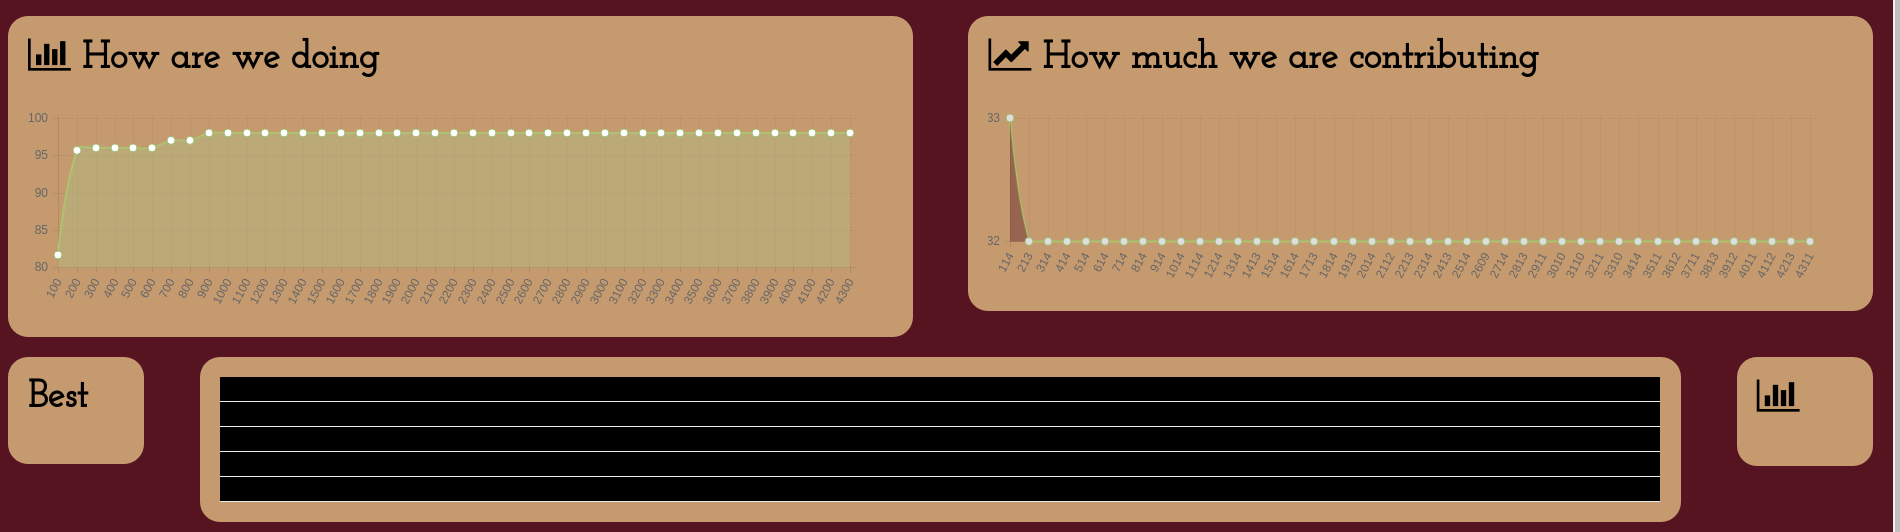
\includegraphics[width=0.95\linewidth]{finish.png}
\caption{The three panels showing the latest fitness, the cache size
  and the best chromosome using 4 shades from white to black to
  represent the number of ones in every block in the Trap
  problem at the top; at bottom, the finished algorithm showing 5
  black bars indicating that the 50 traps have been found. \label{fig:all}}
\end{figure*}

\begin{figure}[!htb]
\centering
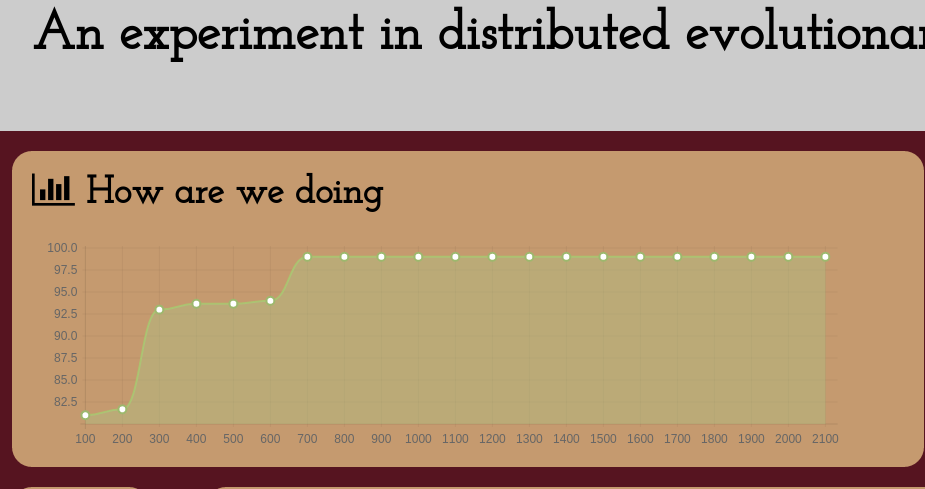
\includegraphics[width=0.95\linewidth]{fitness.png}
\caption{This panel, labeled with ``How are we doing'', shows
  the evolution in time of the fitness, it rotates to show only the
  last 5000 generations.  \label{fig:fitness}}
\end{figure}

\begin{figure}[!htb]
\centering
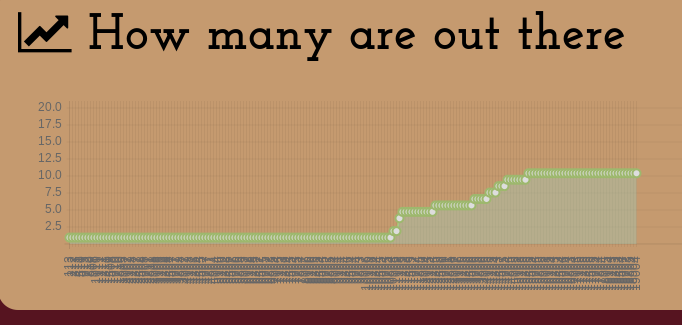
\includegraphics[width=0.95\linewidth]{howmany.png}
\caption{This panel, labeled with ``How many are out there'', shows
  the number of different IPs that are contributing to the simulation,
  accumulated since the beginning of the simulation run.  \label{fig:howmany}}
\end{figure}

\begin{figure}[!htb]
\centering
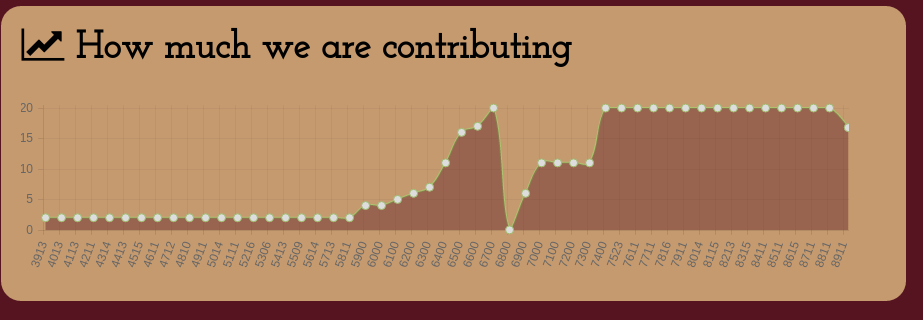
\includegraphics[width=0.95\linewidth]{contribution.png}
\caption{This panel, labeled with ``How much I am contributing'', in
  fact shows the cache size. Cache increases when new individuals are
  added to the pool; it stays the same if the users keep sending the
  same individuals. The graph shows the activity of the last 5000
  generations in a rotating fashion, eliminating the first as new ones
  arrive.  \label{fig:howmuch}}
\end{figure}




%---------------------------------------------------------------
\section{Conclusions and future work}
\label{sec:conclusion}


%---------------------------------------------------------------
\section*{Acknowledgment}
 
This work has been supported in part by
TIN2014-56494-C4-3-P (Spanish Ministry of Economy and Competitivity), PROY-PP2015-06 (Plan Propio 2015 UGR). Additional support was received by
Projects 5622.15-P (ITM) and  PROINNOVA 2015: 220590 (CONACYT).

\bibliographystyle{abbrv}
\bibliography{geneura,volunteer,javascript,pool}

\end{document}

%%% Local Variables:
%%% ispell-local-dictionary: "english"
%%% End:
